\documentclass[a4paper,11pt]{article}

%%%%%%%%%%%%%%%%%%%%%%%%%%%%%%%%%%%%%
% STD PACKAGES
%%%%%%%%%%%%%%%%%%%%%%%%%%%%%%%%%%%%%

\usepackage{amsthm,amsmath,amssymb,amsfonts}
\usepackage{marginnote}
\usepackage{enumerate}
\usepackage[colorlinks,citecolor=red]{hyperref}

\usepackage{subfigure}


%%%%%%%%%%%%%%%%%%%%%%%%%%%%%%%%%%%%%
% TIKZ
%%%%%%%%%%%%%%%%%%%%%%%%%%%%%%%%%%%%%

\usepackage{tkz-euclide}
\usetikzlibrary{patterns}
\usetikzlibrary{calc}
\usetikzlibrary{positioning}
\usetikzlibrary{decorations.pathmorphing}
\tikzstyle{point}=[draw,circle,fill=black,scale=.3] %draws a point call as \coordinate[point]
\tikzset{baseline={([yshift=-.5ex]current bounding box.center)}, every picture}

%%%%%%%%%%%%%%%%%%%%%%%%%%%%%%%%%%%%%
% THEOREMS
%%%%%%%%%%%%%%%%%%%%%%%%%%%%%%%%%%%%%

\theoremstyle{definition}
\newtheorem{remark}{Remark}

%%%%%%%%%%%%%%%%%%%%%%%%%%%%%%%%%%%%%
% CUSTOM COMMANDS
%%%%%%%%%%%%%%%%%%%%%%%%%%%%%%%%%%%%%

\makeatletter
\newcommand*{\defeq}{\mathrel{\rlap{%
    \raisebox{0.3ex}{$\m@th\cdot$}}%
  \raisebox{-0.3ex}{$\m@th\cdot$}}%
=}
\makeatother

\newcommand{\hooklongrightarrow}{\lhook\joinrel\longrightarrow}
\newcommand{\hooklongleftarrow}{\longleftarrow\joinrel\rhook}


\newcommand{\NN}{\mathbb{N}}
\newcommand{\ZZ}{\mathbb{Z}}
\newcommand{\QQ}{\mathbb{Q}}
\newcommand{\RR}{\mathbb{R}}
\newcommand{\CC}{\mathbb{C}}
\newcommand{\CP}{\mathbb{CP}}
\newcommand{\HH}{\mathbb{H}}
\newcommand{\DD}{\mathbb{D}}
\newcommand{\RP}{\mathbb{RP}}

\DeclareMathOperator{\GL}{GL}
\DeclareMathOperator{\SL}{SL}
\DeclareMathOperator{\PSL}{PSL}
\DeclareMathOperator{\SO}{SO}
\DeclareMathOperator{\SU}{SU}
\DeclareMathOperator{\PSU}{PSU}
\DeclareMathOperator{\U}{U}
\DeclareMathOperator{\diag}{diag}

\newcommand{\g}{\mathfrak{g}}
\newcommand{\h}{\mathfrak{h}}
\newcommand{\m}{\mathfrak{m}}
\newcommand{\su}{\mathfrak{su}}

\newcommand{\del}{\partial}
\newcommand{\delbar}{\bar{\partial}}
\newcommand{\F}{\mathcal{F}}
\newcommand{\OO}{\mathcal O}
\newcommand{\M}{\mathcal{M}}
\newcommand{\EE}{\mathcal{E}}
\newcommand{\Tr}{\mathrm{Tr}\,}
\renewcommand{\Im}{\mathrm{Im}}
\renewcommand{\Re}{\mathrm{Re}}
\newcommand{\acton}{\rotatebox[origin=c]{-90}{$\circlearrowright$}}
\newcommand{\ket}[1]{\lvert #1 \rangle}
\newcommand{\bra}[1]{\langle #1 \rvert}

\newcommand{\mat}[4]{\begin{pmatrix} #1 & #2 \\ #3 & #4 \end{pmatrix}}
\newcommand{\vek}[2]{\begin{pmatrix} #1 \\ #2 \end{pmatrix}}

\usepackage{showlabels}

\title{Working Title}
\author{}
\date{\today}

\begin{document}

\maketitle

\tableofcontents

\section{Toy model: \texorpdfstring{$0d$ GLSM}{0d GLSM}}
\subsection{Setup}
We start with a $0d$ GLSM toy model, i.e.\ we consider the source manifold $\Sigma = \{ pt \}$ to be an abstract point and the target manifold to be $$X = \CP^{N-1} \times \CP^{N-1}$$
The space of fields is then simply given by points on the target manifold $X$, namely 
\begin{equation}
  \F = \CP^{N-1} \times \CP^{N-1}
\end{equation}
As the action of the model we consider 
\begin{equation}
  S(z,w) = -\beta \lvert \langle \bar z, w\rangle \rvert^2 = -\beta \sum_{j,k = 0}^{N-1} \bar z_j z_k \bar w_j w_k 
  \label{eq:toy_S}
\end{equation}
where $z,w \in \CC^{N}$ subject to the condition 
\begin{equation}
  \lvert z \rvert^2 = \sum_j \lvert z_j \rvert^2 = 1 \quad , \quad \lvert w \rvert^2 = \sum_k \lvert w_k \rvert^2 = 1
  \label{eq:toy_constr}
\end{equation}
The action enjoys a $\U(1) \times \U(1)$ gauge freedom (which here is simply a global $\U(1) \times \U(1)$ symmetry, acting as 
\begin{equation}
  e^{i\theta}\times e^{i\varphi}\colon (z,w) \mapsto (e^{i\theta} z, e^{i\varphi} w)
\end{equation}
Under the assumption of the condition \eqref{eq:toy_constr}, the action \eqref{eq:toy_S} does define a function on $\CP^{N-1} \times \CP^{N-1}$.

The path integral of the model is defined by 
\begin{equation}
  Z = \int \prod_j dz_j d\bar z_j dw_j d\bar w_j \delta(\lvert z \rvert^2  - 1)\delta(\lvert w \rvert^2 -1)  e^{-S(z,w)}
  \label{eq:toy_Z}
\end{equation}
In order to evaluate \eqref{eq:toy_Z}, we want to embed the space of fields $\mathcal F = \CP^{N-1} \times \CP^{N-1}$ into a higher dimensional complex space such that 
\begin{enumerate}
  \item the new action $\tilde S$ is holomorphic in the new variables (fields)
  \item when we restrict to $\mathcal F$, $\tilde S$ reduces to $S$
\end{enumerate}
We think of this embedding as an analytic continuation of the space of fields in an appropriate sense.

\subsection{Complexification of Real Analytic Manifolds}
Let us first recall a basic construction of complexification of real analytic manifolds due to Bruhat and Whitney \cite{Bruhat_Whitney}.

Let $M$ be a real analytic manifold of dimension $\dim_{\RR} M = m$.
Moreover, let $\{ U_i, \phi_i \}$ be a real analytic atlas of $M$, with $U_i \subset \RR^m$ and charts $\phi_i \colon U_i \to M$ so that the transition functions
\begin{equation}
  \phi_{ij} = \phi_j^{-1} \circ \phi_i \colon U_{ij} \to U_{ij}
\end{equation}
are real analytic diffeomorphisms.
The idea of complexifying $M$ is to find a complex manifold $M^{\CC}$ with $\dim_{\CC} M^{\CC} = m$ and a (real analytic) isomorphism $f\colon M \to \tilde M \subset M^{\CC}$ of $M$ onto a submanifold of $M^{\CC}$. 
(Fancy way to say that $M$ should be a real analytic submanifold of $M^{\CC}$ up to isomorphism)
Now, find opens $U_i^{\CC} \subset \CC^m$ such that $U_i^{\CC} \cap \RR^m = U_i$ and extend the charts $\phi_i$ charts $\phi_i^{\CC}$ such that 
\begin{enumerate}[(i)]
  \item the transition functions $\phi^{\CC}_{ij} \colon U^{\CC}_{ij} \to U^{\CC}_{ij}$ are biholomorphic

  \item $\phi^{\CC}_{ji} = \left( \phi^{\CC}_{ij} \right)^{-1}$ and $\phi^{\CC}_{ii} = id$

  \item the transition functions $\phi^{\CC}_{ij}$ satisfy the usual 2-cocycle condition (gluing condition) on $U^{\CC}_{ijk}$: $\phi^{\CC}_{ij}\circ\phi^{\CC}_{jk} = \phi^{\CC}_{ik}$
\end{enumerate}
These conditions ensure that we can glue $M^{\CC}$ from the local data $\{ U_i^{\CC}, \phi_i^{\CC} \}$:
\begin{equation}
  M^{\CC} = \coprod_i U_i^{\CC} / \sim \quad , \quad z_i \sim z_j \text{~iff~} z_j = \phi^{\CC}_{ji}(z_i) \text{~on~} U^{\CC}_{ij}
\end{equation}

For more details on this construction see \href{https://books.google.ca/books?id=In1Dbj-pkIkC&pg=PA103\&dq=complexification+of+real+analytic+manifolds\&hl=en&sa=X\&ei=aYRAUrWeBYPZ2AWEj4DoBA\&ved=0CD8Q6AEwAQ#v=onepage\&q=complexification\%20of\%20real\%20analytic\%20manifolds&f=false}{Cieliebak and Eliashberga's book} \cite{CEbook}

\subsubsection{Example: The \texorpdfstring{$N$-sphere}{N-sphere}}\label{subsec:cmplxfy_sphere}
Consider the $N$-sphere $S^{N} \subset \RR^{N+1}$.
First, consider the following atlas: let $p_{\pm} = (0, \dots,0, \pm 1) \in S^{N}$ be the north and south pole respectively.
We denote points on the sphere by $x = (x_1, \dots, x_{N+1})$, $\lVert x \rVert^2 = 1$ and points in $\RR^N$ by $X = (X_1, \dots, X_N)$.
The atlas we consider is given by steoreographic projection through $p_{\pm}$:
Let $U_{\pm} = \RR^N$ and $V_{\pm} = S^N - \{ p_{\pm} \}$. 
Then define charts
\begin{equation}
  \phi_{\pm} \colon U_{\pm} \to V_{\pm} \subset S^N \quad , \quad X \mapsto \left( \frac{2 X}{1 + \lVert X \rVert^2}, \pm \frac{\lVert X \rVert^2 - 1}{\lVert X \rVert^2 + 1} \right)
\end{equation}
with inverse
\begin{equation}
  \phi_{\pm}^{-1} \colon x \mapsto \left\{\frac{x_i}{1 \mp x_{N+1}}\right\}
\end{equation}
From this, one finds the transition functions
\begin{equation}
  \phi_{+-} = (\phi_{-+})^{-1} = \phi_{-}^{-1}\circ \phi_{+} \colon X \mapsto \frac{X}{\lVert X \rVert^2}
\end{equation}
\begin{remark}
  There is a nice geometric interpretation of these transition functions.
  Note that the map 
  \begin{equation}
    X \mapsto \frac{X}{\lVert X \rVert^2}
  \end{equation}
  describes an involution at the unit sphere $S^{N-1}$.
  On the sphere, the maps differ merely by a sign switch in the $x_{N+1}$ component and indeed, if one computes the transition functions directly on the embedded sphere (that is as maps from $\RR^{N+1} \to \RR^{N+1}$) one finds
  \begin{equation}
    \phi_{+} \circ \phi_{-} \colon (x_i, x_{N+1}) \mapsto (x_i, - x_{N+1})
  \end{equation}
  which corresponds to a reflection of $x$ about the equator! (It helps visualising this for the case 2-sphere)
  But under stereographic projection, a reflection about the equator becomes an inversion on the unit sphere $S^{N-1}$ in $\RR^N$ (again, it helps working this out in the case $N=2$).
\end{remark}

Now, since $U_{\pm} = \RR^N$ there exist obvious candidates for a complexification, namely $U^{\CC}_{\pm} = \CC^N$. 
We thus promote every $X$ to a complex variable $Z = X + i Y$.
Conversely, we can promote any $x \in \RR^{N+1}$ satisfying $\lVert x \rVert^2 = \sum_j x_j^2 = 1$ to complex variables $z$ satisfying 
\begin{equation}
  \sum_j z_j^2 = 1
  \label{eq:toy_quadric}
\end{equation}
The above equation defines a hypersurface (so-called \emph{quadric}) inside $\CC^{N+1}$.

There is a very interesting observation I found in \href{https://math.stackexchange.com/questions/1784898/tangent-bundle-of-sphere-as-a-complex-manifold}{this} stackexchange post: the quadric $Q$ defined by \eqref{eq:toy_quadric} is \emph{diffeomorphic} to the tangent space $TS^N$.
The diffeomorphism is realised by the following map:
\begin{equation}
  \Psi \colon TS^{N} \to Q \quad , \quad (x,y) \mapsto z = \Psi(x,y) = x \sqrt{1 + \lVert y \rVert^2} + i y
\end{equation}
with inverse 
\begin{equation}
  \Psi^{-1}(x + i y) = \left( \frac{x}{\sqrt{1 + \lVert y \rVert^2}}, y \right) 
\end{equation}
where $\lVert y \rVert^2 = \sum_{i} y_i^2$.
\begin{remark}
Verification that $\Psi$ does indeed define a diffeomorphism goes by a straight forward calculation.
(Recall in particular that the tangent space $TS^N$ can be described by pairs $(x,y) \in \RR^{N+1}$ such that $\langle x, y\rangle = \sum_i x_i y_i = 0$)
\end{remark}

There exists another very interesting diffeomorphism (which I have discovered in this \href{https://math.stackexchange.com/questions/4871752/tangent-bundle-of-a-sphere-t-mathbb-sn-is-diffeomorphic-to-mathbb-sn-time}{stackexchange post}
\begin{equation}
  \Phi \colon S^N \time S^N / \Delta \to TS^N \quad , \quad (u,v) \mapsto \left( u, \frac{v - \left\langle u, v \right\rangle u}{1 - \left\langle u, v \right\rangle } \right)
  \label{eq:diff_SNSN_TSN}
\end{equation}
Its inverse is given by 
\begin{equation}
  \Phi^{-1} \colon TS^N \to S^N \times S^N / \Delta \quad , \quad (x,y) \mapsto \left( x, \frac{x(\lVert y \rVert^2 - 1) + 2 y}{\lVert y \rVert^2 + 1} \right)
\end{equation}
\begin{remark}
  The map \eqref{eq:diff_SNSN_TSN} is the sterepgraphic projection of $v \in S^N$ through the ``pole'' $u \in S^N$.
\end{remark}
Finally we have the following commutative diagram 
\begin{equation}
  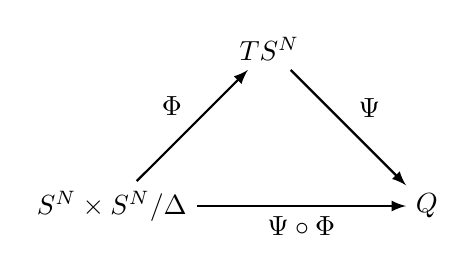
\begin{tikzpicture}
    \node (TS) at (0,2) {$TS^N$};
    \node (SS) at (-2,0) {$S^N \times S^N / \Delta$};
    \node (Q) at (2,0) {$Q$};

    \draw[thick,-{latex}] (SS) -- node[midway,below] {$\Psi\circ\Phi$}(Q);
    \draw[thick,-{latex}] (TS) -- node[midway, above right] {$\Psi$} (Q);
    \draw[thick,-{latex}] (SS) -- node[midway, above left] {$\Phi$} (TS);
  \end{tikzpicture}
\end{equation}

\begin{remark}
  The original $S^N \subset Q$ was located at $S^N = Q \cap \RR^{N+1}$. 
  If we follow this through, we see that this $S^N$ corresponds to the zero section $\{ (x,0) \in TS^N \}$ inside $TS^N$ and consequently is defined by $\Phi(u,v) = (u,0)$ inside $S^N \times S^N / \Delta$.
Note that this is precisely the anti-diagonal 
\begin{equation}
  \bar\Delta = \{ (u,-u) \mid u \in S^N \} \subset S^N \times S^N
\end{equation}
Indeed, the stereographic projection of $-u$ (``south pole'') through $u$ (``north pole'') gives zero:
\begin{equation}
  -u \mapsto \frac{(-u) - \left\langle (-u),u \right\rangle u}{1 - \left\langle (-u), u \right\rangle } = \frac{-u + \lVert u \rVert^2 u}{1 + \lVert u \rVert^2} = 0
\end{equation}
since $\lVert u \rVert^2 = 1$.
Hence 
\begin{equation}
  \Phi(u,-u) = (u,0)
\end{equation}
and the original $S^N$ is located along the anti-diagonal $\bar\Delta$. 
\end{remark}

\subsection{Factor from \texorpdfstring{$\delta$}{delta}-function Constraint}
Recall that we are interested in integrals of the form 
\begin{equation}
  I = \int_{\CP^n \times \CP^n} d\mu(z) d\mu(w) e^{-S(z,w)} \OO(z,w)
\end{equation}
where $d\mu(z) = \prod_i dz_i d\bar z_i$ and we have included some observable $\OO \colon \CP^n \to \CC$.
For our toy model, we consider the action functional \eqref{eq:toy_S}
\begin{equation}
  S(z,w) = -\beta \lvert \langle \bar z, w\rangle \rvert^2   
\end{equation}
It is instructive pass to real coordinates.
If $z_k = a_k + i b_k$, let $x_k$ be the real vector $(a_k\ b_k)^t$.
If we collect all components, we can form the real vector $x = ( \dots a_k\ b_k \dots)^t \in \RR^{2n +2}$.
We denote the real vector associated to $w$ by $y$.
In terms of these, the path integral over can be written as 
\begin{equation}
vol(S^1)^2\int_{\RR^{2n + 2} \times \RR^{2n + 2}} d^{2n + 2}x\ d^{2n + 2y}\ \delta(\lVert x \rVert^2 - 1)\delta(\lVert y \rVert ^2 -1) e^{- S(x,y)}\OO(x,y)
\end{equation}
where the pre-factor stems from the compact part of the gauge group $\CC^* \acton \CC^{n+1}$.
Let us focus on the following part of the integral:
\begin{equation}
  I \sim \int_{\RR^{2n + 2}} \delta(\lVert x \rVert^2 - 1) = \int_{\RR^{2n + 2}} \delta(\left\langle x, x \right\rangle  - 1) 
\end{equation}
Following our idea, we complexify the space of integration, $x \to \zeta$
\begin{equation}
  I \sim \int_{\Gamma_0 = \RR^{2n + 2} \cap \CC^{2n + 2}} \delta(\left\langle \zeta, \zeta \right\rangle  - 1)
\end{equation}
where 
\begin{equation}
  \left\langle \zeta, \zeta \right\rangle = \sum_k \zeta_k^2
\end{equation}
The $\delta$-function constraint restricts the support of the integrand to the quadric $Q$.
Now, we would like to deform the ``contour'' (domain of integration) inside $Q$
\begin{equation}
   I \sim \int_{\Gamma_a \subset \CC^{2n + 2}} \delta(\left\langle \zeta, \zeta \right\rangle  - 1)
\end{equation}
Inspired by the discussion in \ref{subsec:cmplxfy_sphere}, we would like to parametrise $Q$ in terms of $TS^{2n + 1}$.
We thus choose a parametrisation of the following form: (by abuse of notation, we will use again $x$ to denote a vector in $\RR^{2n + 2}$)
\begin{equation}
  \zeta(x) = x \sqrt{1 + \lVert y(x) \rVert^2} + i y(x)
  \label{eq:parametrisation}
\end{equation}
where $y(x)$ is chosen in such a way that $\left\langle x,y \right\rangle = 0$.
It follows that 
\begin{equation}
  I \sim \int_{\RR^{2n + 2}} d^{2n + 2}x\ \det J(x) \delta(\langle \zeta(x), \zeta(x) \rangle - 1)
\end{equation}
where $J(x)$ denotes the Jacobian of \eqref{eq:parametrisation}.
Note that the $\delta$-function constraint can be simplified as follows: Let 
\begin{equation}
  \lambda(x) = \sqrt{1 - \lVert y \rVert^2}
\end{equation}
Then 
\begin{equation}
  \begin{split} 
    C(x) &= \left\langle \zeta(x), \zeta(x) \right\rangle  - 1 \\
    &= \lambda^2(x) \lVert x \rVert^2 + 2 i \lambda(x) \left\langle x, y(x) \right\rangle  - \lVert y \rVert^2 - 1\\
    &= \lambda^2(x) (\lVert x \rVert^2 - 1)
  \end{split}
\end{equation}
Importantly, 
\begin{equation}
  \lambda^2(x) > 0 
\end{equation}
such that the $\delta$-function constraint is of the following form:
\begin{equation}
  \begin{split} 
    \int \delta(C(x)) &= \int d\mu(x) \delta(\underbrace{f(x)g(x)}_{\equiv\phi(x)}) \\
    &= \int_{\phi^{-1}(0)}\frac{d\sigma}{\lVert \nabla \phi(x) \rVert} \\
    &= \int_{f^{-1}(0)} \frac{d\sigma}{\lVert f(x) \nabla g(x) + g(x) \nabla f(x) \rVert } \\
    &= \int_{f^{-1}(x)} \frac{d\sigma}{\lVert \nabla f(x) \rVert}\frac{1}{\lvert g(x) \rvert} \\
    &= \int d\mu \frac{\delta(f(x)}{\lvert g(x) \rvert}
  \end{split}
\end{equation}
where $f(x) = \lVert x \rVert^2 - 1$ and  $g(x) = \lambda^2(x) > 0$.
Hence we find that with the chosen parametrisation, the integral nicely localises to an integral over $S^{2n + 1}$
\begin{equation}
  \int_{\RR^{2n + 2}} \delta(C(x)) = \int_{\RR^{2n+2}} \frac{\delta\left( \lVert x \rVert^2 - 1 \right)}{\lambda^2(x)} = \int_{S^{2n + 1}} \frac{1}{\lambda^2(x)}
\end{equation}
Therefore, we are left with an integral of the form 
\begin{equation}
  I \sim \int_{S^{2n + 1}} \frac{\det J(x)}{\lambda^2(x)} \quad , \quad \lambda^2(x) = 1 + \lVert y(x) \rVert^2
  \label{eq:toy_schema_I}
\end{equation}

\subsection{Homogeneous Deformations}

\subsubsection{Example: \texorpdfstring{$n=0$}{n=0}}

A particular nice example, which can be computed explicitly and serves as a check that everything works nicely is given for the case $n=0$.
Consider the deformation 
\begin{equation}
  y(x) = \alpha \Omega x \quad , \quad \lVert x \rVert^2 = 1\quad , \quad \Omega = \mat{0}{1}{-1}{0} \in \SO(2) \quad , \quad \alpha \in \RR
  \label{eq:toy_cst_def}
\end{equation}
so that indeed 
\begin{equation}
  \left\langle x, y(x) \right\rangle = 0
\end{equation}
Moreover, note that 
\begin{equation}
  \lVert y(x) \rVert^2 = \left\langle y(x), y(x) \right\rangle = \alpha^2 \left\langle x, \Omega^t \Omega x \right\rangle = \alpha^2 \lVert x \rVert^2 = \alpha^2
\end{equation}
and hence 
\begin{equation}
  \lambda^2(x) = 1 + \alpha^2
\end{equation}
We compute the Jacobian of this parametrisation as follows: let $M_{i}^{\;j} = \del_i y^j(x)$.
Then 
\begin{equation}
  \begin{split} 
    J_i^{\;j} = \lambda(x) \delta_{i}^{\;j} + \frac{\left\langle y, \del_i y \right\rangle x^j}{\lambda(x)} + i M_i^{\;j} =  \lambda(x) \delta_{i}^{\;j} + \frac{M_{ik}y^k x^j}{\lambda(x)} + i M_i^{\;j}
  \end{split}
\end{equation}
Using bra-ket notation and trivially lowering indices (considering the flat metric on $\RR^2$), we can write $J$ as follows:
\begin{equation}
  J = \lambda(x) \cdot id + \lambda^{-1}(x) \ket{My}\bra{x} + i M
\end{equation}
\begin{remark}
  The matrix $M$ has some interesting properties.
  \begin{enumerate}
    \item From $\left\langle x, y(x) \right\rangle = 0$ it follows that
      \[
      0 = \del_i \left\langle x, y(x) \right\rangle = y_i(x) + M_{ik} x_k
      \] 
      so that 
      \[
	y_i(x) = M_{ik} x_k \implies y(x) = Mx
      \] 
      and hence
      \[
	\left\langle x, y \right\rangle = \left\langle x , Mx \right\rangle = \left\langle M^t x, x \right\rangle = 0
      \] 
      from which follows (if $y(x) = Mx \neq 0$)
      \[
	\bra{x} M = 0
      \] 
  \end{enumerate}
\end{remark}
Now, for our choice of
\[
  y(x) = \alpha \Omega x
\] 
we have
\begin{equation}
  M = \alpha \Omega^t = - \alpha \Omega
\end{equation}
and hence 
\begin{equation}
  \begin{split} 
    J &= \lambda(x) \cdot id + \lambda^{-1}(x) \alpha^2 \Omega^t \Omega \ket{x} \bra{x} - i \alpha \Omega \\
    &= \lambda(x) \cdot id + \lambda^{-1}(x) \alpha^2 \ket{x} \bra{x} - i \alpha \Omega
  \end{split}
\end{equation}
Now, here is a neat trick due to Tej.
Consider the unitary matrix 
\begin{equation}
  U = (x\ \Omega x) \quad , \quad \Omega^{*} = \begin{pmatrix} x^t \\ x^t \Omega^t \end{pmatrix}
\end{equation}
where $x$ is a $2\times 2$ column vector with unit norm.
Then 
\begin{equation}
  U^* U = \mat{\left\langle x, x \right\rangle}{\left\langle x, \Omega x \right\rangle}{\left\langle \Omega x, x \right\rangle}{\left\langle x, x \right\rangle} = \mat{1}{0}{0}{1}
\end{equation}
Moreover,
\begin{equation}
  \bra{x} U = x^t U = (\left\langle x,x \right\rangle\  \left\langle x, \Omega x \right\rangle) = (1\ 0)
\end{equation}
as well as
\begin{equation}
  U^* \Omega U = U^* (\Omega x\ \Omega^2 x) = U^* (\Omega x\ -x) = \mat{\left\langle x, \Omega x \right\rangle}{-\left\langle x, x \right\rangle}{\left\langle x, \Omega^t\Omega x\right\rangle}{-\left\langle x, \Omega^t x \right\rangle} = -\Omega
\end{equation}
Then
\begin{equation}
  \begin{split} 
    U^* J U &= \lambda(x) \cdot id + \lambda^{-1}(x) \alpha^2 U^* \ket{x}\bra{x} U - i\alpha U^* \Omega U \\
    &= \lambda(x) \cdot id + \lambda^{-1}(x) \alpha^2 U^* \mat{1}{0}{0}{0} + i\alpha \Omega \\
    &= \mat{\lambda(x) + \lambda^{-1}(x) \alpha^2}{i\alpha}{-i\alpha}{\lambda(x)}
  \end{split}
\end{equation}
It follows that 
\begin{equation}
  \begin{split} 
    \det J(x) &= \det( U^* J(x) U) \\
    &= \det \mat{\lambda(x) + \lambda^{-1}(x) \alpha^2}{i\alpha}{-i\alpha}{\lambda(x)} \\
    &= \lambda^2(x) + \alpha^2 - \alpha^2 = \lambda^2(x)
  \end{split}
\end{equation}
Finally, we obtain that
\begin{equation}
  I \sim \int_{S^{2n+1}} \frac{\det J(x)}{\lambda^2(x)} = \int_{S^{2n+1}} \frac{\lambda^2(x)}{\lambda^2(x)} = \int_{S^{2n+1}}
\end{equation}
This means that the \emph{constant deformation} \eqref{eq:toy_cst_def} comes with a trivial \emph{total} Jacobian (Jacobian + factor from the $\varphi$-function constraint).

\subsubsection{The General Case}
The $n=0$ example can be nicely generalised. 
Tej suggested to consider deformations of the form
\begin{equation}
  Y_a(X) = \Omega(a) X \quad , \quad \Omega(a) = \diag\left( \mat{0}{-a_1}{a_1}{\hphantom{-}0}, \dots, \mat{0}{-a_{n+1}}{a_{n+1}}{\hphantom{-}0} \right)
  \label{eq:Tej_deformation}
\end{equation}
for some $a = (a_1, \dots, a_{n+1}) \in \RR^{n+1}$.
This type of deformation have a very nice geometric origin, as we now explain.
\begin{remark}
  Under the isomorphism 
  \begin{equation}
    \RR^{2n + 2} \cong \CC^{n+1} \quad , \quad \vek{x_k}{y_k} \mapsto z_k = x_k + i y_k
  \end{equation}
  the deformation \eqref{eq:Tej_deformation} is acting on $\CC^{n+1}$ by multiplication with the diagonal matrix $\diag(i a_1, \dots, i a_{n+1})$
    \begin{equation}
      \begin{pmatrix} \vdots \\ z_k \\ \vdots \end{pmatrix} \mapsto \begin{pmatrix} \vdots \\ i a_k z_k \\  \vdots \end{pmatrix} 
    \end{equation}
    The finite diffeomorphism generated by this vector field is given by 
    \begin{equation}
      \begin{pmatrix} \vdots \\ z_k \\ \vdots \end{pmatrix} \mapsto \begin{pmatrix} \vdots \\ e^{i a_k} z_k \\  \vdots \end{pmatrix} 
    \end{equation}
    The generated finite action is thus the action of the torus 
    \begin{equation}
      U(1)^{n+1} \subset \SU(n+1)
    \end{equation}
\end{remark}

Let $G$ be a Lie group and $H < G$ a subgroup with Lie algebras $\g$ and $\h$ respectively.
The orbit space $G/H$ is known as a \emph{homogeneous space}. 
It is called \emph{reductive} if $\g$ allows the following decomposition
\begin{equation}
  \g = \h \oplus \m \quad , \quad [\h,\h] \subset \h \quad , \quad [\h,\m] \subset \m
\end{equation}
If $\g$ is equipped with a Killing form $B$ (or if $G$ allows a $G$-invariant metric as a manifold), then $G/H$ is automatically reductive with the choice 
\begin{equation}
  \m = \h^{\perp}
\end{equation}
where $\h^{\perp}$ is the orthogonal to $\h$ with respect to $B$.
Indeed, since $B$ is $G$-invariant, schematically
\begin{equation}
  0 = B(\h,\m) = B([\h,\h],\m) = B(\h,[\h,\m])
\end{equation}
so that $[\h,\m] \subset \m$.

In summary, given a reductive homogeneous space $G/H$, we get a nice decomposition of the tangent space: first, let $o = [e]$ be the class in $G/H$ at the identity.
Then 
\begin{equation}
  T_o(G/H) \cong \m
\end{equation}
This isomorphism is given essentially by the pushforward of the natural projection $\pi \colon G \to G/H$.
In fact, $\pi \colon G \to G/H$ defines a principal $H$-bundle. 
Its vertical vector fields are given by $\ker(\pi_*) = \h$ and since $\pi$ is a submersion ($\pi$ and $\pi_*$ are both surjective) we have
\begin{equation}
  \pi_* \colon \g / \ker(\pi_*) = \g / \h \cong T_o(G/H)
\end{equation}
Then, to compute the tangent space at any other point, we use translation by $G$.

Now, recall that 
\begin{equation}
  S^{2n + 1} = \SU(n+1) / \SU(n)
\end{equation}
is a homogeneous space where $H = \SU(n)$ sits inside $G = \SU(n+1)$ as the lower right corner
\begin{equation}
  \SU(n) \ni h \hookrightarrow \mat{1}{0}{0}{h} \in \SU(n+1)
\end{equation}
The reductive split is given by 
\begin{equation}
  \su(n+1) = \su(n) \oplus \m
  \label{eq:red_split}
\end{equation}
Since $\su(n+1)$ admits a Killing form $B(x,y) \propto tr(x,y)$, we can choose $\m = \su(n)^{\perp}$.
In the split \eqref{eq:red_split}, we have 
\begin{equation}
  \su(n) \equiv \mat{0}{0}{0}{\su(n)} \subset \su(n+1)
\end{equation}
We then find 
\begin{equation}
  \m = \su(n)^{\perp} = \left\{ \mat{0}{-\zeta^*}{\zeta}{0} \right\} \quad , \quad \zeta \in \CC^{n+1}
\end{equation}
Here $\zeta^* = \bar \zeta^t$ denotes the hermitian conjugate. 

In order to describe the tangent space $T_{[g]}(G/K)$ at any point $[g] \in G/H$, we can use the tangential map of left translations. 
In fact, left translation by $g$ is defined by the map
\begin{equation}
  L_g \colon G \to G \quad , \quad g' \mapsto g g'
\end{equation}
so that its tangential map
\begin{equation}
  \theta_g = (L_{g^{-1}})_* \colon T_g G \to T_e G = \g
\end{equation}
This map defines a $\g$-valued 1-form on $G$ known as the left-invariant Maurer-Cartan form. 
For a matrix group, it can be written as 
\begin{equation}
  \theta_g = g^{-1}dg
\end{equation}
Note that the natural projection $\pi \colon G \to G/H$ is equivariant with respect to left translation: if 
\begin{equation}
  \tau_g \colon G/H \to G/H \quad , \quad [g'] \mapsto [gg']
\end{equation}
then we have
\begin{equation}
  \pi \circ L_g = \tau_g \circ \pi \quad , \quad \tau_g\circ\tau_{g'} = \tau_{gg'}
\end{equation}
Moreover, 
\begin{equation}
  (\pi\circ L_{g^{-1}})_* = \pi_* \circ (L_{g^{-1}})_* = (\tau_{g^{-1}} \circ \pi)_* = (\tau_{g^{-1}})_* \circ \pi_*
\end{equation}
Hence, denoting $(\tau_{g^{-1}})_* = \vartheta_g$, we have
\begin{equation}
  \pi_* \circ \theta_g = \vartheta_g \circ \pi_* \colon T_g G \to T_{o}(G/H) = \m
\end{equation}
For us, we will be mainly interested in the map
\begin{equation}
  (\tau_g)_* \colon \m = T_{[e]}(G/H) \to T_{[g]}(G/H)
\end{equation}
which parametrises the tangent space of $G/H$ at a point $[g]$ by $\m$.

Now, if $G$ is a matrix group the pushforward $(\tau_g)_*$ is essentially just given by left multiplication with $g$ (matrix multiplication is linear) and so in we could describe the tangent space $T_p(G/H)$ at a point $p = g(p) p_0$ as follows
\begin{equation}
  T_p(G/H) \cong \{ (p,g(p) \xi) \mid \xi \in \m \} 
\end{equation}
where we implicitly identify $g(p) X$ with $g(p) X p_0$.


\begin{remark}
  In theory, this is very nice. 
  In practice, I believe it is computationally expensive: for a given $p \in S^{2n +1} = \SU(n+1)/\SU(n)$, we would need to find $g(p)$ which on top of it is only defined up to a multiplication on the right of $\SU(n)$.
  We could, for example, choose $p_0 = (1,0\dots)^t$.
  There is a way how to algorithmically compute $g(p)$: A matrix belongs to $\SU(n+1)$ iff its columns (rows) form an orthonormal basis of $\CC^{n+1}$.
  If $p_0 = e_1$ is the first standard basis vector, then we start with the basis $\{ p, e_2,\dots, e_{n+1} \}$ and by Gram-Schmidt produce an orthonormal basis $\{ p, \tilde e_1, \dots, \tilde e_{n+1} \}$ and set
  \begin{equation}
    g(p) = (p\; \tilde e_2\; \dots; \tilde e_n)
  \end{equation}
  However, I believe that Gram-Schmidt is computationally expensive.

  Moreover, it might simply not be necessary.
  In order to define interesting deformations, we could simply consider any $X \in \g$.
  Any such $\xi$ will admit a split into $\xi = \xi_{\m} + \xi_{\h}$ and since $\h = \text{Lie}(H) \cong \text{Stab}(p)$ is in the Lie algebra of the stablizer of $p$ (\emph{note that we actually mean $p$ here, not $p_0$}), $\xi_h p = 0$ (as $hp = p$ for any $h$ in $H$).
  Thus, we could simply not care and just work with $X$ as a whole and define deformations for any $\xi\in\g$ by 
  \begin{equation}
    Y_{\xi}(X) = \rho(\xi)\cdot X \quad , \quad \xi \in \g \quad , \quad X \in S^{2n + 1} 
  \end{equation}
  Here, $\rho$ denotes the appropriate representation of $\g$ on $S^{2n+1}$.
  I believe its easiest description is as follows: $\SU(n+1)$ and hence $\su(n+1)$ naturally acts (by matrix multiplication) on $S^{2n+1}$ when viewed as a subset of $\CC^{n+1}$. 
  Under the isomorphism $\CC \cong \RR^2$, where $z = x + iy \mapsto (x, y)$, multiplication by a complex number $a + i b$ becomes matrix multiplication:
  \begin{equation}
    (a + i b) z \iff \mat{a}{-b}{b}{a} \vek{x}{y}
  \end{equation}
  Hence, using our representation of $\CC^{n+1}$
  \begin{equation}
    \begin{pmatrix} \vdots \\ z_k = x_k + i y_k \\ \vdots \end{pmatrix} \mapsto \begin{pmatrix} \vdots \\  x_k \\ y_k \\ \vdots \end{pmatrix}
  \end{equation}
  we have to simply replace any complex number $a + i b$ in $\xi \in \su(n+1)$ by the appropriate matrix:
  \begin{equation}
    \rho(\xi) \colon a + i b \leadsto \mat{a}{-b}{b}{a}
  \end{equation}
  In practice, it might be easier to have the following workflow:
  \begin{equation}
    \begin{matrix}
      S^{2n+1} \subset \RR^{2n + 2} & \longrightarrow & \CC^{n+1} & \stackrel{\xi \cdot}{\longrightarrow} & \CC^{n+1} & \longrightarrow & \RR^{2n + 2} \\
      X & \longrightarrow & Z & \stackrel{\xi \cdot}{\longrightarrow} & \xi \cdot Z & \longrightarrow & Y_{\xi}(X)
    \end{matrix}
  \end{equation}
\end{remark}

\begin{thebibliography}{99}
  \bibitem{Bruhat_Whitney} F.\ Bruhat and H.\ Whitney, Quelques propri\'et\'es fondamentales des ensembles analytiques-r\'eels, Comment. Math. Helv. 33, 132-160 (1959).

  \bibitem{CEbook} K.\ Cieliebak and Y.\ Eliashberg. From Stein to Weinstein and back: symplectic geometry of affine complex manifolds. Vol. 59. American Mathematical Soc., 2012.
\end{thebibliography}
\end{document}
